\chapter{Future work and limitations}

\section{Introduction}

In this chapter we present the limitations and possible improvements of FrDataFlow. 
The current implementation is rather limited in its functionality because we wanted to focus on the mapping layer and the possibilities of parallelization using the dataflow engine.
However, multiple improvements can still be made. The setup of signals is still a rigid system in that it does not allow the dynamic creation of new signals, the filtering of values or just generally manipulating the timing of value propagation. Every signal always has to emit a value for every set of incoming values. While this already allows for a rich set of programs, these manipulations would be necessary to implement any non trivial program using FrDataFlow. 

\section{Dynamically creating signals}

One of the common patterns in reactive programming is the dynamic creation of new signals based on some state or external input.
In a web environment, imagine a program that searches a database while the user types keywords. This stream of text can be represented as a signal that is attached to the text input field and emits strings upon every keystroke. Then we create a child signal which subscribes which takes these strings and launches an XMLHTTPRequest (ajax request) to fetch the data that satisfies these keywords. Every request again can be modeled as a signal which emits the data that is retrieved and then goes silent. Essentially what this program is doing is dynamically creating a new signal (XMLHTTPRequest) for every value in another signal (the keystrokes). To take this example even further, when the user types another character, we would like to discard any previously created XMLHTTPRequests because we no longer care for their results. Ideally, some sort of cancellation could happen if it is not already too late, but we definitely want to ignore any data that is retrieved based on outdated keywords. This means our dynamically added signals are not only quickly created, but also discarded.

An implementation of this pattern can be observed in the RxJs\footnote{In RxJs, a signal is known as an \textit{observable}. When signals dynamically produce more signals, they are called \textit{higher order observables}.} library. \citep{_observable_2017}. It contains the \textit{switch} operator, which is visually represented by figure \ref{fig:futurework-dynamicsignals-switch}.

\begin{figure}[h!]
	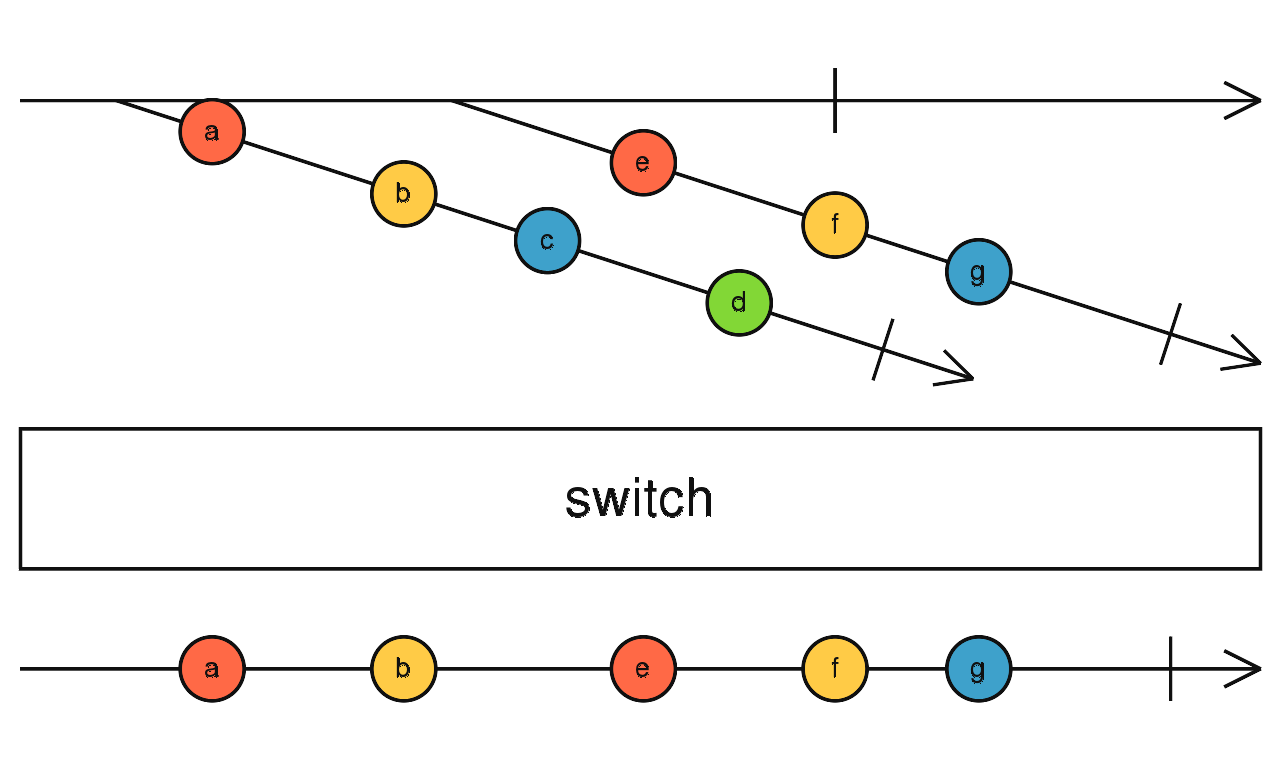
\includegraphics[width=\textwidth]{images/FutureWork-DynamicSignals-Switch.png}
	\caption{A timeline diagram of the \textit{switch} operator in RxJs}
	\label{fig:futurework-dynamicsignals-switch}
\end{figure}

In this figure, we can see a top horizontal arrow which represents the root signal. Values of this signal are transformed into child signals, which on their part can again emit multiple values. 
Since we are only interested in the latest data, we essentially \textit{unsubscribe} from the first child signal when a new value appears in the root signal, so that the sample values c and d never propagate to the end result. 

In the current version of FrDataFlow, it is unfortunately not possible to create new signals at runtime. A possible improvement would be to allow this, which would mean the signal would have to be added to the topologically sorted signals and be translated to a dataflow node. This would also mean that any existing dataflow nodes upon which this new signal depends would have to be updated to also generate tokens for this new node. Similarly, upon destroying signals, this node and all the references to it would have to be updated.

\subsection{Filtering}

Another common practice is filtering of signals, only letting values through which satisfy a certain predicate. Our current implementation of FrDataFlow models signals as a mapping function which takes a set of inputs and produces a new value for every updated set. Filtering would introduce the possibility of not propagating a value at all if certain criteria are not met. In essence, a signal would no longer provide a lambda that has to return a value, but a lambda that can push values into a type of sink when it wants to. This refactoring would allow for a whole category of powerful constructs, such as taking only the first n values, throttling signals, etc. 

An example visualization of the filter function in RxJs can be seen in figure  \ref{fig:futurework-filtering-filter}. 

\begin{figure}[h!]
	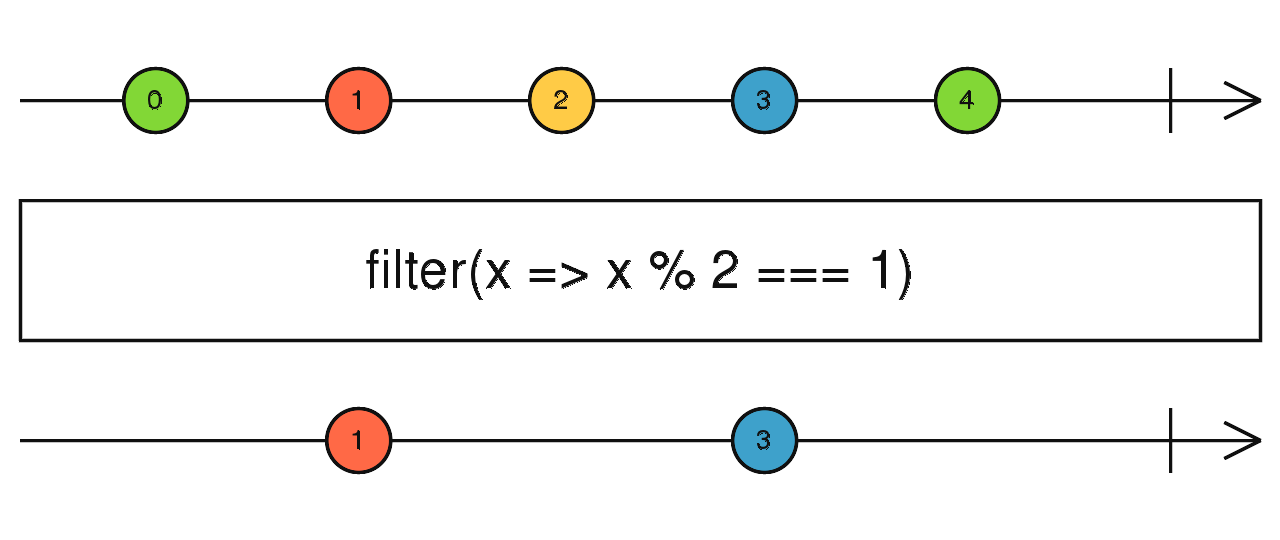
\includegraphics[width=\textwidth]{images/FutureWork-Filtering-Filter.png}
	\caption{A timeline diagram of the \textit{filter} operator in RxJs}
	\label{fig:futurework-filtering-filter}
\end{figure}

We see at the top a signal which produces a stream of numbers. If we create a new signal that filters these numbers using the filter function, we get a new stream of numbers that only contains those that satisfied the predicate. When the number 0 is pushed into the signal lambda, it does not propagate it into the sink of the child signal, which means the value does not go through. 

To implement this pattern in our mapping layer, we would have to ensure that dataflow nodes don't always have to produce new tokens when they are invoked, and a way for nodes to indicate when this should happen or not. However, there is no technical reason why the dataflow engine should not be able to handle this: it is simply the presence of tokens that determines which nodes are invoked, so not emitting these tokens would essentially implement the filtering behavior we have described.


\section{Conclusion}

In this chapter we have shown how FrDataFlow is still a basic language that does not support some powerful concepts such as the dynamic creation of signals or the filtering of values.
If these concepts were to be introduced, they would allow for an implementation of most of the techniques commonly found in other reactive libraries or languages.

This initial version of FrDataFlow has focused mostly on the practical mapping layer from reactive programming to the dataflow model. There are however no immediate technical shortcomings that should prevent us from implementing the modifications presented in this chapter.